% Figura 5 — Ciclo fechado proposto (alinhado ao Artigo; NAO implementado no NOC Lite)
% Fonte: arquitetura_sistema.md, Sec. 6.3 (fechamento do ciclo). Tracejado = ausente no sistema.
% Corrigido (Chris): text width + align=center nos estilos box/prop para evitar
% truncamento nas caixas superiores; minimum width maior e reespacamento em x.
\documentclass[tikz,border=4pt]{standalone}
\usepackage{tikz}
\usetikzlibrary{arrows.meta,positioning,shapes.geometric,calc}
\begin{document}
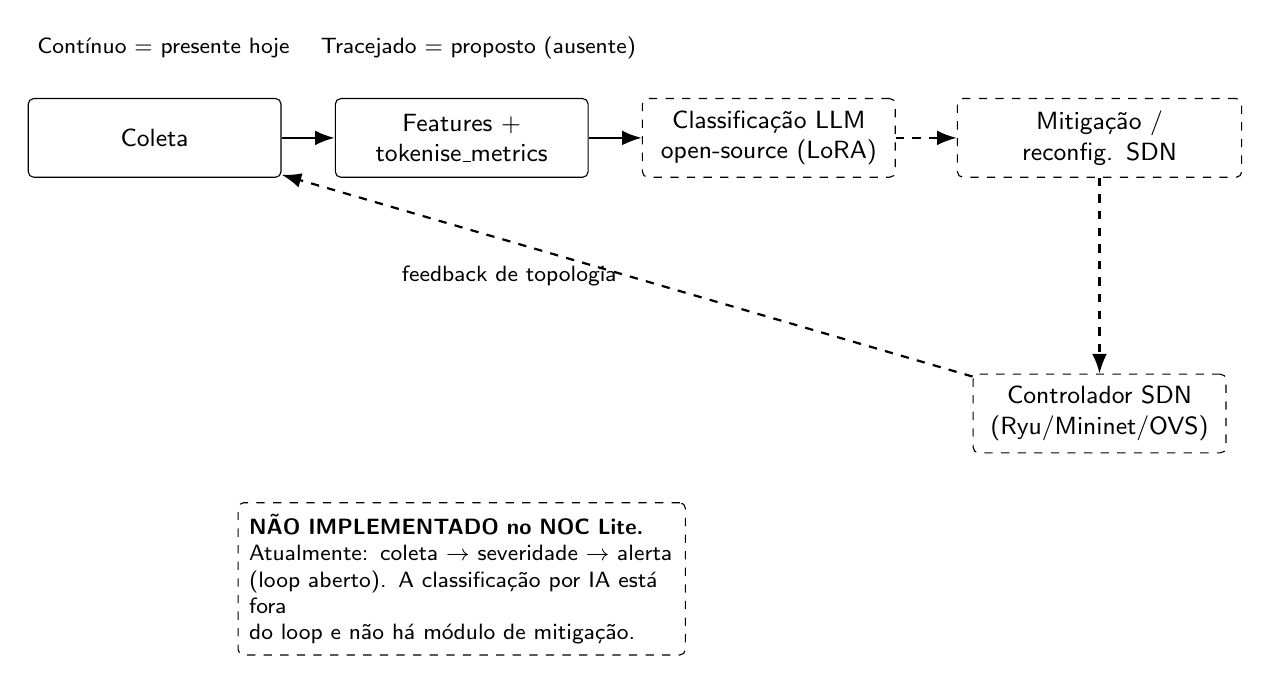
\begin{tikzpicture}[
    font=\sffamily\small,
    box/.style={rectangle, draw=black, rounded corners=2pt,
                minimum width=3.2cm, minimum height=1.0cm,
                text width=3.0cm, align=center, fill=white, inner sep=3pt},
    prop/.style={rectangle, draw=black, dashed, rounded corners=2pt,
                 minimum width=3.2cm, minimum height=1.0cm,
                 text width=3.0cm, align=center, fill=white, inner sep=3pt},
    arrow/.style={-{Latex[length=2.5mm]}, thick, draw=black},
    darrow/.style={-{Latex[length=2.5mm]}, thick, draw=black, dashed},
  ]

  \node[box]  (col) at (0,4.0)  {Coleta};
  \node[box]  (feat)at (3.9,4.0){Features +\\tokenise\_metrics};
  \node[prop] (cls) at (7.8,4.0){Classificação LLM\\open-source (LoRA)};
  \node[prop, text width=3.4cm, minimum width=3.6cm] (mit) at (12.0,4.0){Mitigação /\\reconfig. SDN};

  \node[prop] (sdn) at (12.0,0.5){Controlador SDN\\(Ryu/Mininet/OVS)};

  % ciclo
  \draw[arrow] (col)  -- (feat);
  \draw[arrow] (feat) -- (cls);
  \draw[darrow] (cls) -- (mit);
  \draw[darrow] (mit) -- (sdn);
  \draw[darrow] (sdn) -- node[left,font=\sffamily\footnotesize]{feedback de topologia} (col);

  % anotacao
  \node[rectangle, draw=black, dashed, rounded corners=2pt,
        text width=5.4cm, inner sep=4pt, font=\sffamily\footnotesize, align=left]
        at (3.9,-1.6) {
        \textbf{NÃO IMPLEMENTADO no NOC Lite.}\\
        Atualmente: coleta $\rightarrow$ severidade $\rightarrow$ alerta\\
        (loop aberto). A classificação por IA está fora\\
        do loop e não há módulo de mitigação.
        };
  \node[font=\sffamily\footnotesize,anchor=north west] at ($(col.north west)+(0,0.9)$)
        {Contínuo = presente hoje \quad Tracejado = proposto (ausente)};
\end{tikzpicture}
\end{document}
